\documentclass[tikz,border=8pt]{standalone}
\usepackage{fontspec}
\setmainfont{TeX Gyre Heros}
\usepackage{amsmath}
\usepackage{unicode-math}
\setmathfont{TeX Gyre Termes Math}
\usetikzlibrary{arrows.meta}
\definecolor{maroon}{HTML}{780404}
\definecolor{orange}{HTML}{E37D00}
\definecolor{charcoal}{HTML}{303238}
\begin{document}
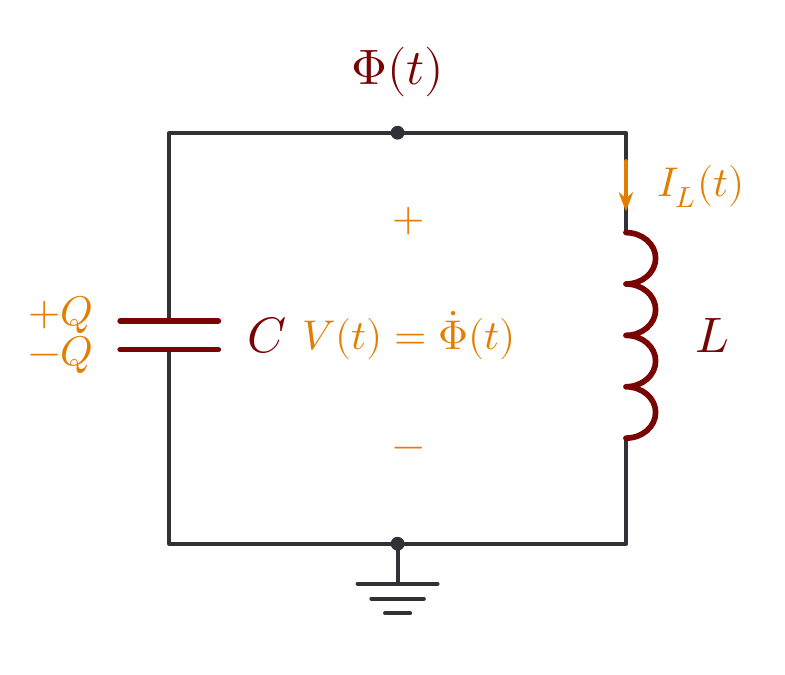
\begin{tikzpicture}[
  x=1.45cm,y=1.45cm,
  line cap=round,line join=round,
  wire/.style={draw=charcoal,line width=1.45pt},
  component/.style={draw=maroon,line width=2.05pt},
  annotation/.style={text=orange,font=\fontsize{15}{18}\selectfont},
  partlabel/.style={text=maroon,font=\fontsize{18}{21}\selectfont},
  text=charcoal
]
% Transparent canvas with balanced margins. No background rectangle is drawn.
\path[use as bounding box] (-1.24,-.90) rectangle (5.15,4.52);

% Both components share exactly two nodes: the upper node and reference ground.
\draw[wire] (0,1.95) -- (0,3.6) -- (4,3.6) -- (4,2.725);
\draw[wire] (0,1.70) -- (0,0) -- (4,0) -- (4,.925);

% Capacitor: upper and lower conducting plates, separated by a real gap.
\draw[component] (-.43,1.95) -- (.43,1.95);
\draw[component] (-.43,1.70) -- (.43,1.70);
\node[partlabel,anchor=west] at (.60,1.825) {$C$};
\node[annotation,anchor=east] at (-.58,2.00) {$+Q$};
\node[annotation,anchor=east] at (-.58,1.65) {$-Q$};

% American inductor symbol: four connected, equally spaced semicircular lobes.
% Each lobe begins and ends at x=4; adjoining lobes are electrically continuous.
\draw[component] (4,2.725)
  arc[start angle=90,end angle=-90,x radius=.26,y radius=.225]
  arc[start angle=90,end angle=-90,x radius=.26,y radius=.225]
  arc[start angle=90,end angle=-90,x radius=.26,y radius=.225]
  arc[start angle=90,end angle=-90,x radius=.26,y radius=.225];
\node[partlabel,anchor=west] at (4.52,1.825) {$L$};

% Current reference enters the positive terminal of L: passive sign convention.
\draw[draw=orange,line width=1.55pt,-{Stealth[length=7pt,width=5.2pt]}]
  (4,3.35) -- (4,2.91);
\node[annotation,anchor=west] at (4.19,3.13) {$I_L(t)$};

% Node flux is an electrical node coordinate, not magnetic flux through the loop.
\fill[charcoal] (2,3.6) circle[radius=2.5pt];
\node[partlabel,anchor=south] at (2,3.83) {$\Phi(t)$};

% Voltage annotation has no connecting line and cannot be mistaken for a branch.
\node[annotation] at (2.10,2.83) {$+$};
\node[annotation] at (2.10,1.825) {$V(t)=\dot{\Phi}(t)$};
\node[annotation] at (2.10,.80) {$-$};

% Common reference node and the conventional three-bar ground symbol.
\fill[charcoal] (2,0) circle[radius=2.5pt];
\draw[wire] (2,0) -- (2,-.35);
\draw[wire] (1.65,-.35) -- (2.35,-.35);
\draw[wire] (1.77,-.48) -- (2.23,-.48);
\draw[wire] (1.89,-.61) -- (2.11,-.61);
\end{tikzpicture}
\end{document}
